\documentclass[%
aip,
jmp,
reprint,
floatfix,
nobibfootnote,
]{revtex4-1}

\usepackage{graphicx}% Include figure files
\usepackage{dcolumn}% Align table columns on decimal point
\usepackage{bm}% bold math
\usepackage{float}
\usepackage{siunitx}
\usepackage{hyperref}
\usepackage{listings}
\usepackage{ gensymb }
%\usepackage[mathlines]{lineno}% Enable numbering of text and display math
%\linenumbers\relax % Commence numbering lines
\usepackage{subcaption}
\usepackage{color}

\definecolor{dkgreen}{rgb}{0,0.6,0}
\definecolor{gray}{rgb}{0.5,0.5,0.5}
\definecolor{mauve}{rgb}{0.58,0,0.82}

\lstset{
	frame=single, 
	language=Python, 
	columns=flexible,
	basicstyle={\small\ttfamily},
	keywordstyle=\color{blue},
	commentstyle=\color{dkgreen},
	stringstyle=\color{red},
	title=\lstname
}

\renewcommand{\arraystretch}{1.3} % Changes the height of tables
\DeclareSIUnit{\pixel}{pix.}


\begin{document}
	
	\title[Scale and FOV Calculations Using Albireo]{Scale and Field of View Calculations Using Albireo}
	
	\author{Lucas, Miles}
	\author{Brandon, John}
	\affiliation{Iowa State University}
	
	\date{\today}
	
	
% Write here a short abstract (1 paragraph) describing what you achieved in this lab.

	\begin{abstract}
	
	We used images of Albireo with an assumed angular separation of $\Delta\alpha = \SI{35.3}{\arcsecond}$ to determine the pixel scale and field of view for our SBIG CCD camera and Meade 8" telescope. We accomplished this by subtracting median dark frames from our raw images and using the DAO star-finding algorithm to find the stars' centroids. Our pixel scale was determined to be \SI{1.0072+-0.0091}{\arcsecond\per\pixel} and our field of view was $\SI{770.50+-0.20}{\arcsecond}\times\SI{513.67+-0.13}{\arcsecond}$. Analyzing our images further there was a difference in the mean and median brightness between \SI{0.1}{\second}, \SI{0.5}{\second}, and \SI{1.0}{\second} exposure times but very little difference in brightness between photometric V, B, and I filters. 
		
	\end{abstract}
	
	\maketitle
%________________________________________________________________________
	
%	Write here a summary of the goals of this lab. Be brief – do not exceed the end of the first page.

	\section{Introduction}
	
	This lab seeks to quantify the pixel scale and field of view of the images taken using the SBIG CCD camera and Meade 8" telescope at the Zaffarano Hall observation deck. To do t his we will take images of sources with a known angular separation. The source we used was Albireo ($\beta$ Cygni), a binary system in the northern sky. Albireo's coordinates are ($19^h30^m43.286^s$, \ang{+27;57;34.84}) with angular separation between the two stars $\Delta\alpha=\SI{35.3}{\arcsecond}$.
	
	To determine the pixel scale from an image, we must find the distance between the two sources. If we have two centroids and we allow $\vec{r}$ to be their separation, then the pixel scale will be
	\begin{equation}
		pixel\ scale = \frac{\Delta\alpha}{||\vec{r}||}
		\label{eqn:pscale}
	\end{equation}
	and the field of view in one direction will be 
	\begin{equation}
		FOV = N \frac{\Delta\alpha}{||\vec{r}||}
		\label{eqn:fov}
	\end{equation}
	where $N$ is the number of pixels in the given direction.
	
	We will also compare the images from each filter and exposure time using their statistical moments to analyze the differences in brightness.
	
%________________________________________________________________________	

%	Describe your telescope and camera setup. For the first lab you should describe the setup in more details. Subsequent labs can refer to the procedure described in the first lab, and focus more on the data acquisition itself. Important details to write include: which stars have been observed, which filters were used (BVI), what exposure times and what calibration procedures have been followed (e.g., dark frames acquisition, photometric standards observed, etc.). Mention also the observing conditions (weather, moon presence, temperature, etc.). You should include the observing log appendix A (a table or a scan of a hardcopy). This section can be as long as necessary, but you should strive for brevity (you can refer to the lab guide to avoid repeating all steps, but make sure you explain anything you did differently, problems encountered, etc.). Use tables to summarize information clearly.

	\section{Data Acquisition and Setup}
	Observations were made on \date{30 August 2017} at the Zaffarano Hall observation deck in Ames, Iowa. The night was very clear and the ambient temperature was around \SI{32}{\degreeCelsius}. Observations were made using a Meade 8" reflector telescope with an SBIG ST-402ME CCD camera with internal V, B, and I filters. 
	
	To setup the telescope we used the Meade's GPS functionality to automatically calibrate its position. This calibration involved using two point sources as guides and orienting the telescope centered on the point source. For these measurements, the calibration sources were Arcturus and Altair. We used a \SI{32}{\milli\meter} eyepiece for our calibration alignment. Using the Meade selector, we navigated to the $\beta$ Cygni system We then switched to a \SI{9}{\milli\meter} eyepiece for fine-alignment on our target. Once we were well centered on our target we removed the eyepiece and inserted our CCD camera.
	
	Using CCDops we selected the V filter and began focusing the CCD camera with a manual knob on the telescope. The exposure time for these focusing grabs was \SI{0.05}{\second}. We based our focus on maximizing the peak amplitude read out in CCDops. We took multiple images at multiple exposures with different filters, all recorded in \autoref{table:log}. For each image grab, we set up an autograb using CCDops and took the frames. At each exposure level, we also took dark frames using autograb in order to reduce systematic error.
%________________________________________________________________________

%Describe what you did to analyze the data. For the first lab this section will be minimal. For subsequent labs you should describe in detail the steps you did to analyze the data.  If applicable you can attach the code you used to analyze the data in Appendix B (either a log of your IDL section, or the code of any scripts you wrote). You can also attach screenshots of your computer session if it helps your discussion. Include tables of raw data in this section. The goal of this section is to describe unambiguously what you did to derive your final images and measured quantities from the raw data. Again be brief but complete (use as much space as you need).
	\section{Data Analysis}
	
	Our analysis included some simple image processing and then used machine learning to determine the pixel scale and field of view. 
	
	Our processing pipeline involved finding median dark frames for each exposure length and then subtracting the dark frames from each science image. We use median dark frames rather than mean because we wanted to avoid outliers in the form of cosmic rays or dark pulses. To create the median images, we used a python script that utilizes numpy's array operations for getting the median of the data arrays from each FITS file. Once we saved the three median dark frames (\SI{0.1}{\second}, \SI{0.5}{\second}, \SI{1.0}{\second}) we used AstroImageJ to automate the subtraction for the 26 science images. A comparison of the science images before and after subtraction is shown in \autoref{fig:comparison}. As you can see, the thermal excitation caused by the camera's electronics is removed. 
	
	To calculate the pixel scale of our image, we need to find the center of each star. To do this, we turned to a machine-learning algorithm that uses Gaussian mixture models for detecting stars. The DAO algorithm was used as part of a python package photutils. For more information on this algorithm, see Stetson \cite{1987PASP...99..191S}. The centroid of each star is reported and was then used to calculate separation and the subsequent measurements of interest. The script is shown in \autoref{lst:measurement}. An example of the centroids calculated using the DAO algorithm is shown in \autoref{fig:centroids}.
	
	\begin{figure}[]
		\begin{subfigure}{\linewidth}
			\centering
			
\includegraphics[width=.8\linewidth]{figs/pre.png}
			\caption{Raw science image}
		\end{subfigure}
		\begin{subfigure}{\linewidth}
			\centering
			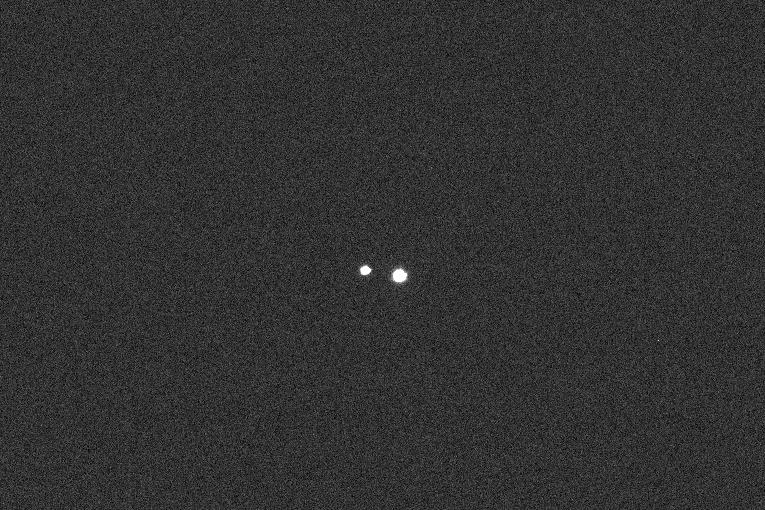
\includegraphics[width=.8\linewidth]{figs/post.png}
			\caption{Processed science image}
		\end{subfigure}
		\caption{Comparison of the raw and processed science images of Albireo in photometric V at \SI{0.1}{\second} exposure.}
		\label{fig:comparison}
	\end{figure}

	\begin{figure}
		\centering
		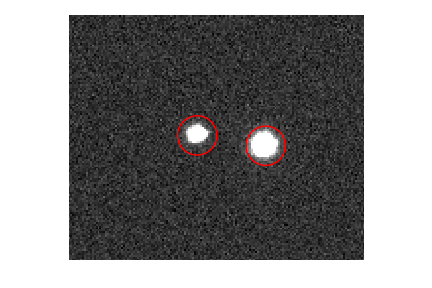
\includegraphics[width=\linewidth]{figs/dao.png}
		\caption{Results of the DAO algorithm on one of the photometric V \SI{0.1}{\second} exposure}
		\label{fig:centroids}
	\end{figure}

%________________________________________________________________________
	
%	Describe in detail the results you obtained from the quantitative analysis of your data, as explained in the lab guide.
	\section{Results}
	 
	 The results of the script are shown in \autoref{table:results}. The mean, median, and standard deviation for each photometric filter and exposure time are listed in \autoref{table:stats}.
	 
	 \begin{table}
	 	\centering
	 	\caption{Pixel scale and field of view values from the 10 photometric V \SI{0.1}{\second} exposures}
	 	\begin{tabular*}{.7\linewidth}{@{\extracolsep{\fill}}c c}
	 		\hline
	 		 Variable   & Value                                     \\ \hline\hline
	 		Pixel Scale & \SI{1.0072+-0.0091}{\arcsecond\per\pixel} \\
	 		   FOV x    & \SI{770.50+-0.20}{\arcsecond}             \\
	 		   FOV y    & \SI{513.67+-0.13}{\arcsecond}             \\ \hline
	 	\end{tabular*}
 		\label{table:results}
	 \end{table}
 
	 \begin{table}
	 	\centering
	 	\caption{The statistics for each photometric filter at each exposure level}
	 	\begin{tabular*}{0.8\linewidth}{@{\extracolsep{\fill}}c r r r r}
	 		\hline
	 		Filter & Exposure          & Max   & Mean & Median \\ \hline\hline
	 		     V & \SI{0.1}{\second} & 19800 & 1.84 & 1.00   \\
	 		     V & \SI{0.5}{\second} & 64500 & 7.56 & 3.00   \\
	 		     V & \SI{1.0}{\second} & 64500 & 13.7 & 6.00   \\
	 		     B & \SI{0.1}{\second} & 23100 & 1.95 & 1.00   \\
	 		     I & \SI{0.1}{\second} & 23100 & 1.95 & 1.00   \\ \hline
	 	\end{tabular*}
	 	\label{table:stats}
	 \end{table}
	
%________________________________________________________________________
	
%	Add here anything else you want to say, and summarize your results. This section should be very brief, not more than a couple of paragraphs
	\section{Conclusions}
	
	The results in \autoref{table:results} show that our CCD camera is able to capture almost exactly one arcsecond per pixel, which gives a field of view of $\SI{771}{\arcsecond}\times\SI{514}{\arcsecond}$. 
	
	Looking through the different processed science images do not show a huge difference between the three photometric filters and the three different exposure times. However, the statistics shown in \autoref{table:stats} show that the longer exposures are brighter, but that there is not much difference between the three filters. We also noted that the \SI{0.5}{\second} and \SI{1.0}{\second} exposures were overexposed as shown by the maximum values corresponding with the maximum values of the CCD. 
	
%________________________________________________________________________
	
	\section*{Acknowledgments}
	
	Thank you to Dr. Charles Kerton and Brandon Marshall for their guidance and assistance in this work.
	
	\section*{References}
	
	\bibliography{refs}
	
	
%________________________________________________________________________
	
	\onecolumngrid
	\appendix
	\section{Observation Log}
	
	\begin{table}[H]
		\centering
		\caption{Observed 06 September 2017 by Miles Lucas and John Brandon}
\begin{tabular}{clclcccl}
	\hline
	Time  & File                   & N Frames & Object                                     & Filter &     Exposure     &       Camera Temp.        & Notes       \\ \hline\hline
	21:39 & M39\_2\_V\_13s\_       &    5     & M39 Objects x1, x4, x7, and x9; stars E, D &   V    & \SI{13}{\second} & \SI{5.33}{\degreeCelsius} &             \\
	21:41 & M39\_2\_V\_13s\_dark\_ &    5     & M39 Objects x1, x4, x7, and x9; stars E, D &   V    & \SI{13}{\second} & \SI{5.33}{\degreeCelsius} & Dark frames \\
	21:43 & M39\_2\_B\_13s\_       &    5     & M39 Objects x1, x4, x7, and x9; stars E, D &   B    & \SI{13}{\second} & \SI{5.33}{\degreeCelsius} &             \\ \hline
\end{tabular}

		\label{table:log}
	\end{table}
%________________________________________________________________________
	
	\section{Analysis Scripts}
	\lstinputlisting[label={lst:measurement}]{../src/measurements.py}
	

\end{document}
%
% ****** End of file aipsamp.tex ******
